\documentclass[UTF8, xcolor=table]{beamer}
\usepackage[BoldFont,SlantFont]{xeCJK}
% \setCJKmainfont[BoldFont={Adobe Heiti Std},ItalicFont={Adobe Kaiti Std}]{AdobeSongStd-Light}
% \setCJKmainfont[BoldFont={AdobeHeitiStd-Regular},ItalicFont={AdobeKaitiStd-Regular}]{AdobeSongStd-Light}
\setCJKmainfont[BoldFont={SimHei},ItalicFont={KaiTi}]{SimSun}
% \setCJKmainfont[BoldFont={Adobe Heiti Std},ItalicFont={Adobe Kaiti Std}]{SimSum} %Windows先编译使用这个字体

\usepackage{latexsym,amssymb,amsmath,amsbsy,amsopn,amstext,xcolor,multicol}
\usepackage{graphicx,wrapfig,fancybox}
\usepackage{pgf,pgfarrows,pgfnodes,pgfautomata,pgfheaps,pgfshade}
\usepackage{thubeamer}
\usepackage[backend=bibtex,sorting=none]{biblatex} % [参考文献格式](https://www.sharelatex.com/blog/2013/07/31/getting-started-with-biblatex.html) %mac IEEE not found
\usepackage{array}
\usepackage{bm}
\usepackage{caption}
\RequirePackage[font=footnotesize]{subcaption}
\usepackage{multirow}
\usepackage{booktabs}
\usepackage{tikz}
\usepackage{tikzscale}
\usepackage{animate}

\defbibheading{bibliography}[\bibname]{} %avoid printbibliography 自动生成目录
\addbibresource{../main.bib}
\setbeamertemplate{bibliography item}[text] 

\usepackage{boxedminipage} %for: bvh border
\def\fourgraphicswidth{0.35} %0.3\textwidth

\usepackage{algorithm} %%format of the algorithm
\usepackage{algpseudocode}
\floatname{algorithm}{算法}
\renewcommand{\algorithmicrequire}{\textbf{输入:}} % Use Input in the format of Algorithm
\renewcommand{\algorithmicensure}{\textbf{输出:}} % UseOutput in the format of Algorithm
\algrenewcommand{\algorithmiccomment}[1]{ $//$ #1}

\usepackage{listings}
\renewcommand\lstlistingname{代码}
\renewcommand\lstlistlistingname{代码}

\lstset{framexleftmargin=1.4em,
        xleftmargin=1.8em,
        basicstyle=\ttfamily\small,
        %frame=shadowbox, numberstyle=\tiny, breaklines=true,
        frame=single,
        numberstyle=\tiny, breaklines=true,
        keywordstyle=\color{blue!70}\bfseries,
        %commentstyle=\color{red!50!green!50!blue!50},
        rulesepcolor=\color{red!20!green!20!blue!20},
        numbers=none,fontadjust=true}
\lstdefinelanguage{shader}{morekeywords={uniform, layout, uniform, vec2, vec3, vec4, in, out, gl_Position, dot, flat, int ,float, gl_VertexID, xyz, w, x, y, z, location, version, sampler2DRect, bgr, gl_FragData, texture2DRect, gl_TexCoord,for,xy},morecomment=[l]{//}}

\begin{document}

\setbeamerfont{footnote}{size=\tiny}
\setbeamerfont{caption}{size=\scriptsize}
\setbeamertemplate{caption}[numbered]
\setbeamerfont{subsection in toc}{size=\footnotesize}
\renewcommand*{\bibfont}{\footnotesize}

\graphicspath{{../}}

\title[自适应的强化学习策略更新算法]{自适应的强化学习策略更新算法}
\author[张元胤]{\vskip 20pt 学~~~~~~生:张~元~胤\\\vskip 10pt 指导老师:张~俊~玉}
\institute[中山大学~数学学院~\&~数学与应用数学]{}%{\small \vskip 38pt 电子信息与工程学院~自动化}
\date{} %{\small \vskip -17pt二〇一六年五月}

%% make title %%
\frame{
        \titlepage
        \vspace{-23mm}
}

\frame {
        \frametitle{目录}
        %\begin{multicols}{2}
        \tableofcontents[sections={<1-7>}]
}

%%
% 引言
% 引言是论文正文的开端,应包括毕业论文选题的背景、目的和意义;对国内外研究现状和相关领域中已有的研究成果的简要评述;介绍本项研究工作研究设想、研究方法或实验设计、理论依据或实验基础;涉及范围和预期结果等。要求言简意赅,注意不要与摘要雷同或成为摘要的注解。
%%

\chapter{引言}
\label{cha:introduction}

\section{问题背景}
\label{sec:background}
% What is the problem
% why is it interesting and important
% Why is it hards, why do naive approaches fails
% why hasn't it been solved before
% what are the key components of my approach and results, also include any specific limitations,do not repeat the abstract
%contribution

强化学习(Reinforcement Learning, RL)\cite{ReinforcementLearning2021} \cite{suttonReinforcementLearningIntroduction2018} 是机器学习(Machine Learning,  ML)领域的一部分。不同于监督学习,强化学习不需要带标签的学习样本, 而是利用奖励或惩罚智能体行为的方式间接设定学习目标。 RL 的灵感 \cite{ReinforcementLearning2021} 来源于心理学中的行为主义理论,即有机体如何在环境给予的奖励或惩罚的刺激下,逐步形成对刺激的预期,产生能获得最大利益的习惯性行为。理论上,强化学习可以达到人工智能(Artificial General Intelligence, AGI)\cite{salvadorREINFORCEMENTLEARNINGLITERATURE2020}。

在标准的强化学习 \cite{mnihAsynchronousMethodsDeep2016} 中,有几个重要的概念:智能体(agent),环境(environment),状态(state),动作(action)和奖励(reward)。考虑扫地机器人的场景:机器人通过在房间里移动和执行清扫动作,从而完成任务。如果有多个扫地机器人,如何挑选出“最好”的一个呢?我们可以计算每块地砖的清洁程度,设定合理的评分机制,从而挑选出得分最高的扫地机器人出来。如果从强化学习的角度看待这个问题,扫地机器人是智能体,房间里面的所有事物就是智能体所在的环境,智能体所在位置以及房间的形状、清洁程度就是改环境的状态,移动和执行清理动作是动作,而每块砖的清洁程度的增加量就是奖励,只是我们要训练出一个得分高的扫地机器人,而不是挑选出一个。现实中有很多这样的问题场景,例如棋盘游戏、电子游戏和自动驾驶等。我们抽象出强化学习的理论框架\cite{suttonReinforcementLearningIntroduction2018}:智能体是完成任务的机器,它负责学习和决策,而智能体执行任务过程中应对的外部事物是环境。这些事务之间持续进行交互,智能体选择动作,环境对这些动作做出响应,呈现出新的状态。同时智能体获取一个奖励,智能体的目标是最大化总的奖励。图 \ref{fig:agent-env-interaction} 展示了整个交互的过程,这将在第二章继续讨论。


\begin{figure}[h]
	\centering
	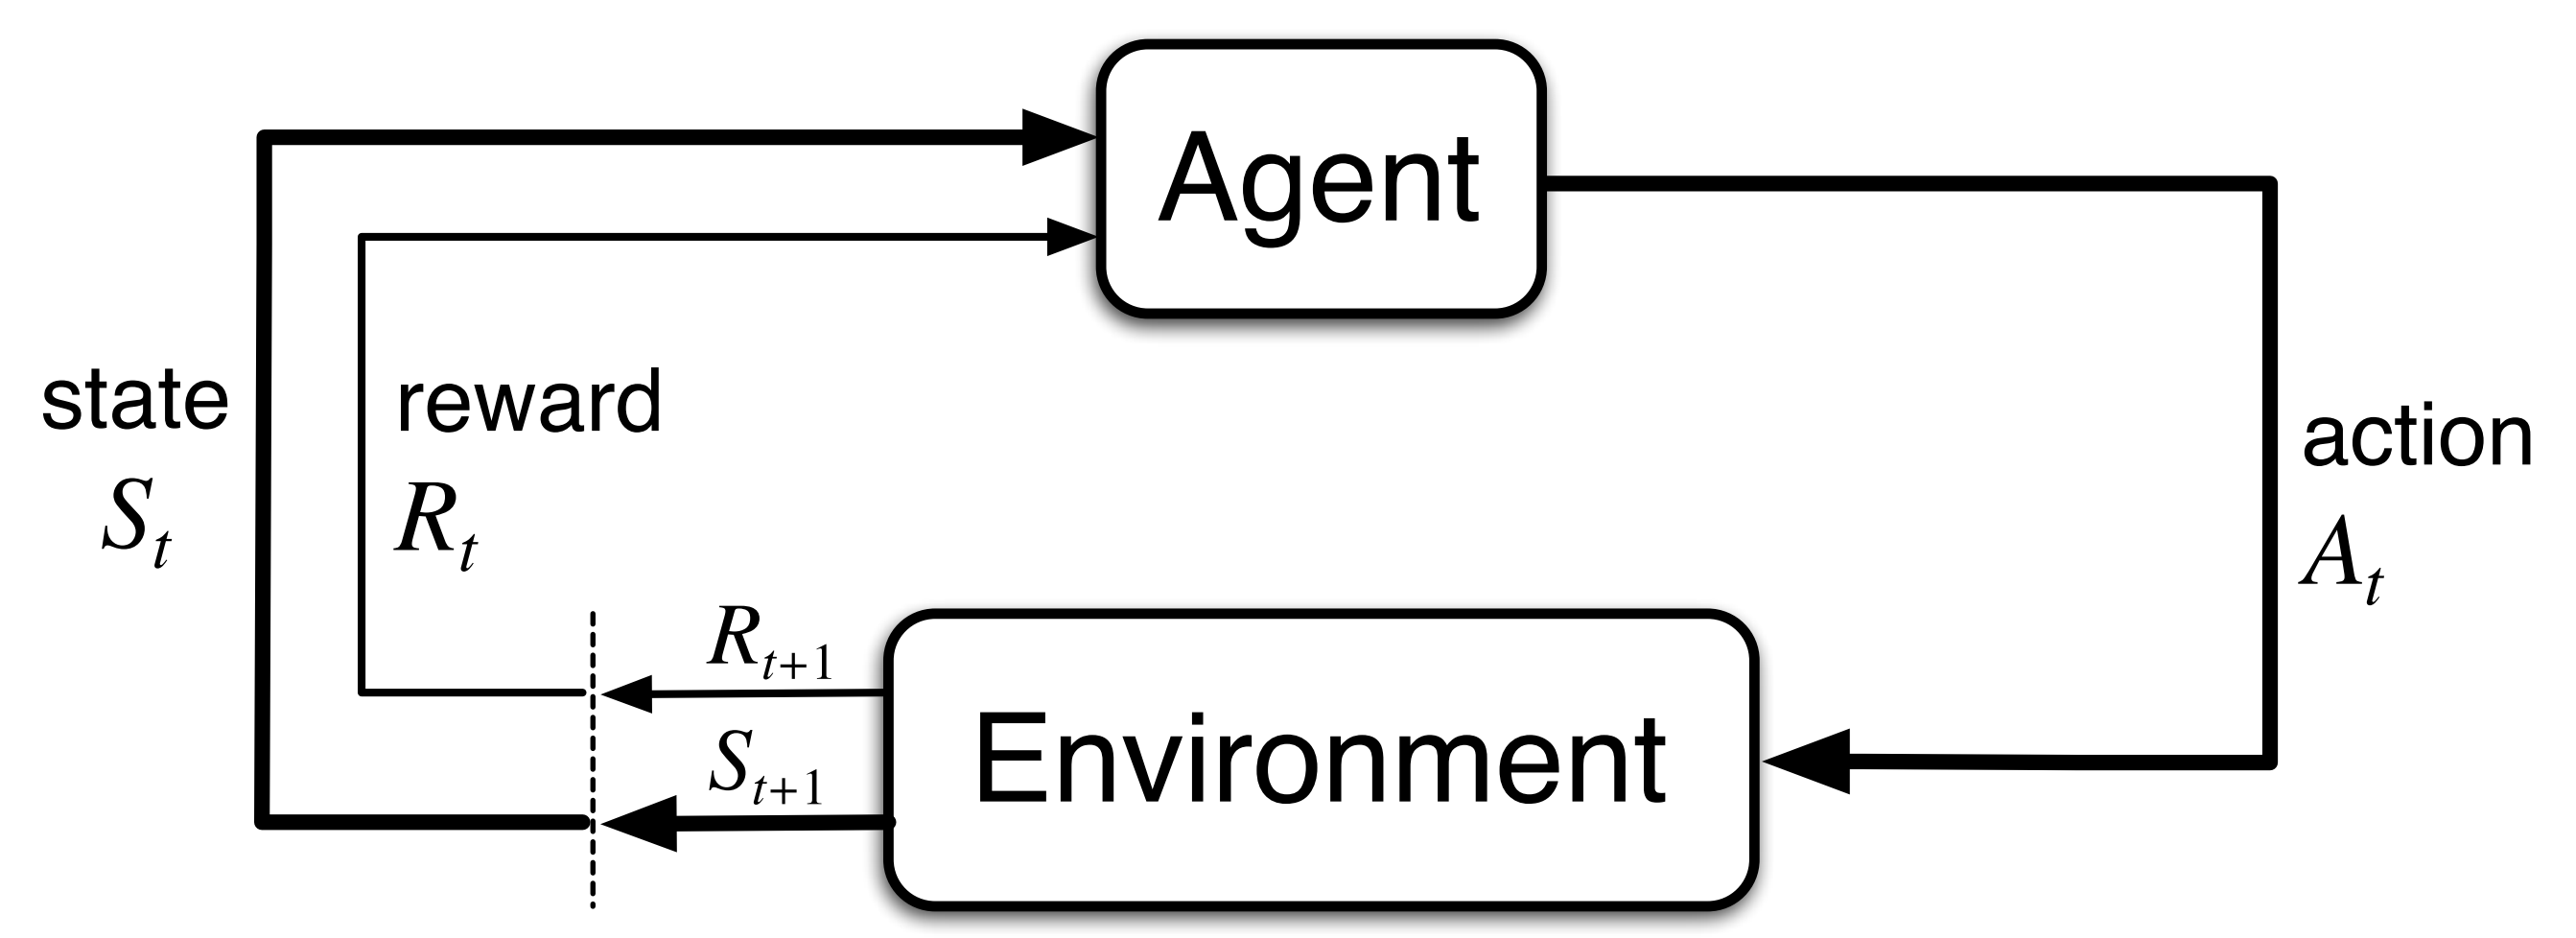
\includegraphics[width=0.9\textwidth]{image/chap01/interaction.png}
	\caption{智能体与环境交互过程\cite{suttonReinforcementLearningIntroduction2018}}
 	\label{fig:agent-env-interaction}
\end{figure}

% \section{强化学习介绍}
在上个世纪,对强化学习的研究已经有很多重要的理论和实践的成果出现\cite{suttonReinforcementLearningIntroduction2018}。过去的强化学习算法主要分为两类,以Q学习算法为代表的基于值函数的方法和以策略梯度算法为代表的基于策略的方法。
近些年来,由于深度学习技术的兴起,强化学习的研究和应用上取得巨大的成就。Mnih 等人提出了DQN 算法\cite{mnihPlayingAtariDeep2013} \cite{mnihHumanlevelControlDeep2015},该算法结合深度学习技术与经典的Q学习算法 \cite{watkinsQlearning1992},使得智能体在 Atari 类游戏能达到人类的控制水平。当然,RL中最令人兴奋的成功案例之一是DeepMind公司开发的AlphaGo \cite{silverMasteringGameGo2016} 和AlphaZero \cite{silverMasteringGameGo2017} 围棋程序。AlphaZero可以玩国际象棋,围棋和其他游戏,相对于仅玩围棋的AlphaGo,它在性能和通用性方面都有改进。这些程序在其他几个方面也很出色。特别是,他们学会了如何在没有人工指导的情况下学会玩游戏。

大部分最近的强化学习相关工作并没有完全脱离原来的研究成果,而是以过去的研究所得的结论为理论基础的 \cite{ohDiscoveringReinforcementLearning2020}。然而,强化学习实践上许多棘手的问题例如稀疏奖励、不完全的状态观察、学习样本不够等等,在根据理想假设的理论上设计的基于值函数或者基于策略的方法并不能很好地解决。本文探索在这些算法的基础上,能否通过机器自动学习到更加适合问题的强化学习算法。


\section{本文的论文结构与章节安排}
\label{sec:arrangement}

本文共分为六章,各章节内容安排如下:第一章提出文章的问题背景,同时介绍强化学习的作用和相关进展。 第二章是背景知识,介绍理解强化学习各个算法所必需的知识点。第三章是文献综述,对与本文方法相关的文献进行整理。第四章是本文算法的详细描述,同时穿插着作者的考量。第五章是本文所提出的方法的实验验证,将本文方法与经典的算法进行对比,然后分析实验结果。第六章总结本文所有的工作,指出本文方法的优点和不足之处,并提出可能做的改进。

\section{背景知识}
\frame
{
	\frametitle{\secname~ }
	\begin{block}{基本概念}
		传统的人工神经网络
	\end{block}
	\begin{block}{Q学习}
		目前最为流行的,广泛应用于视觉任务的神经网络
	\end{block}
	\begin{block}{A2C算法}
		与卷积网络相比,更适用于处理时序信号
	\end{block}
}
\subsection*{基本概念}
\frame{
	\frametitle{前馈神经网络结构}
	\begin{columns}[onlytextwidth]
		\begin{column}{0.5\textwidth}
			\vspace{-1.5em}
			\begin{itemize}
				\item 有向无环图的结构
				\item 输入层(数据特征)
				\item 隐含层(映射后的特征)
				\item 输出层(预测结果)
				\item 反向传播算法(训练方法)
			\end{itemize}
		\end{column}
		\begin{column}{0.5\textwidth}
			% \begin{figure}[h] %structure of LSTM
			% 	\centering
			% 	\includegraphics[width=0.9\textwidth]{image/illustration/network1.pdf}
			% 	\caption{前馈神经网络模型示意图}
			% 	\label{fig:lstm}
			% \end{figure}
		\end{column}
	\end{columns}
}

\frame{
	\frametitle{卷积神经网络}
	\vspace{-0.8em}
	% \begin{figure}
	% 	\centering
	% 	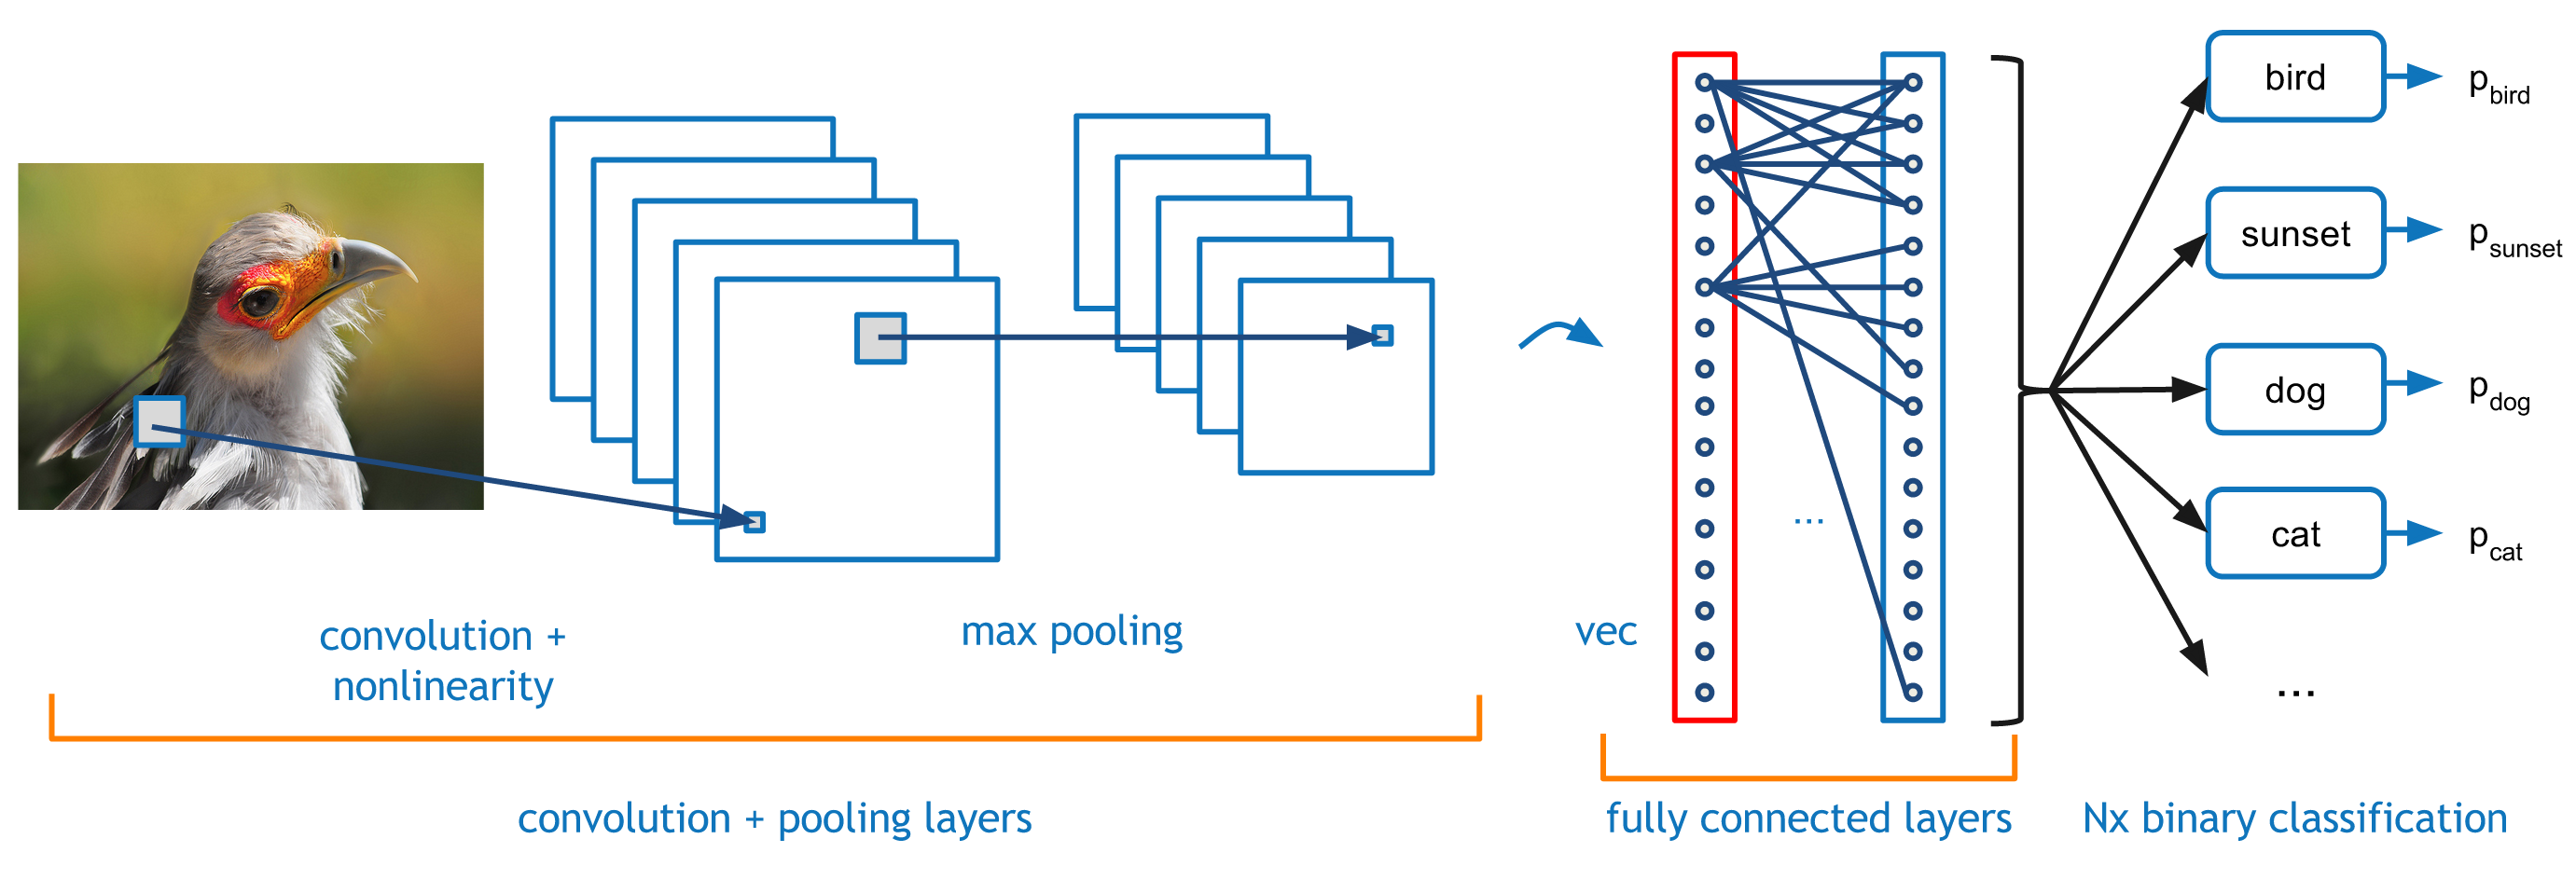
\includegraphics[width=0.8\textwidth]{figures/CNN}
	% 	\caption{卷积网络模型示意图}
	% 	\label{fig:network1}
	% \end{figure}
	\vspace{-0.8em}
	\begin{block}{与前馈神经网络的区别}
		\begin{itemize}
			\item 直接作用于二维图像,无需特征设计阶段
			\item 卷积层,池化层
			\item 局部感知域,权重共享
		\end{itemize}
	\end{block}
}

\frame{
	\frametitle{长短记忆网络(处理一维信号)}
	\tiny
	\vspace{-2em}
	\begin{columns}[onlytextwidth]
		\begin{column}{0.5\textwidth}
			% \begin{figure}[h] %structure of LSTM
			% 	\centering
			% 	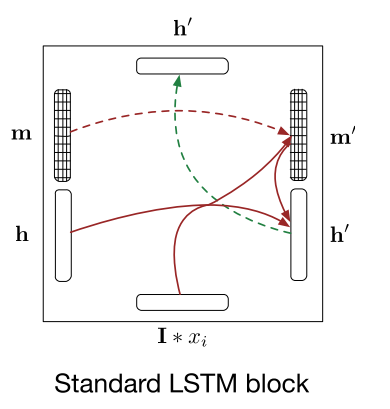
\includegraphics[width=0.6\textwidth]{figures/lstmblock1}
			% 	\caption{长短记忆网络区块示意图}
			% 	\label{fig:lstm}
			% \end{figure}
		\end{column}
		%%%%%%% new column
		\begin{column}{0.5\textwidth}
			\begin{boxedminipage}{0.8\textwidth}
				\vspace{-1.5em}
				\begin{align}
					\label{eq:lstm}
					\begin{split}
						\textbf{g}^u &= \delta(\textbf{W}^u*\textbf{H}) \\
						\textbf{g}^f &= \delta(\textbf{W}^f*\textbf{H}) \\
						\textbf{g}^o &= \delta(\textbf{W}^o*\textbf{H}) \\
						\textbf{g}^c &= \mbox{tanh}(\textbf{W}^c*\textbf{H}) \\
						\textbf{m}' &= \textbf{g}^f \odot \textbf{m} + \textbf{g}^u \odot \textbf{g}^c \\
						\textbf{h}' &= \mbox{tanh}(\bf{g}^o \odot \bf{m}') \\
						\textbf{H} & = \begin{bmatrix}
							I*\textbf{x}_i \\ \textbf{h}
						\end{bmatrix}
					\end{split}
				\end{align}
			\end{boxedminipage}
		\end{column}
	\end{columns}

	\vspace{-1em}
	\begin{block}{缩写形式}
		\footnotesize
		\begin{equation*}
			(\textbf{h}', \textbf{m}') = \mbox{LSTM}\bigr(\textbf{H},\textbf{m},\textbf{W} \bigr)
		\end{equation*}
		其中\textbf{W}包含了四个门权值矩阵$\textbf{W}^u,\textbf{W}^f,\textbf{W}^o,\textbf{W}^c$。
	\end{block}
}

\frame{
	\frametitle{网格型长短记忆网络(处理N维信号)}
	\vspace{-1.5em}
	% \begin{figure}[h]
	% 	\centering
	% 	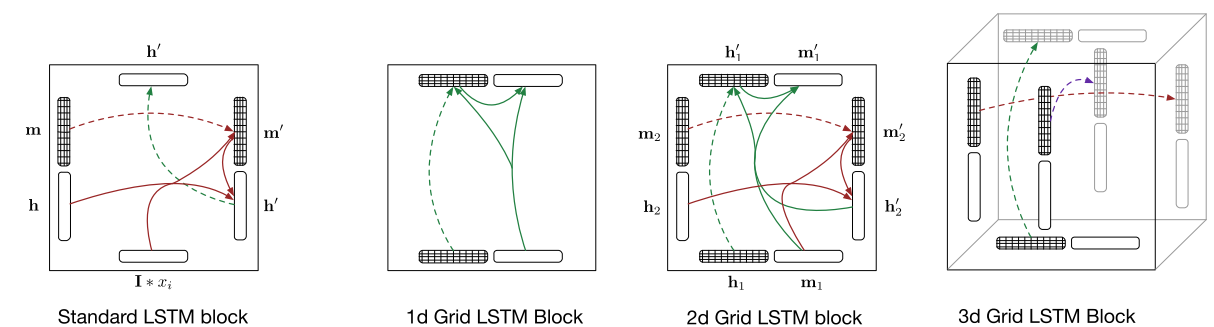
\includegraphics[width=\textwidth]{figures/gridlstm}
	% 	\caption{网格型长短记忆网络区块示意图[Kalchbrenner et al, Grid LSTM, ICLR 2016]}
	% \end{figure}
	\vspace{-2em}
	\begin{block}{网格型长短记忆网络更新过程}
		\tiny
		\begin{columns}[onlytextwidth]
			\begin{column}{0.4\textwidth}
				\vspace{-0.5em}
				\begin{equation}
					\textbf{H} = \begin{bmatrix}
						\textbf{h}_i \\ \vdots \\ \textbf{h}_N
					\end{bmatrix}
				\end{equation}
			\end{column}
			\begin{column}{0.6\textwidth}
				\vspace{-1em}
				\begin{align}
					\begin{split}
						(\textbf{h}_1', \textbf{m}_1') & =  \mbox{LSTM}(\textbf{H}, \textbf{m}_1, \textbf{W}_1) \\ &\mbox{ }\vdots \\
						(\textbf{h}_N', \textbf{m}_N') & =  \mbox{LSTM}(\textbf{H}, \textbf{m}_N, \textbf{W}_N)
					\end{split}
					\label{eq:gridlstm}
				\end{align}
			\end{column}
		\end{columns}
	\end{block}
}
\endinput

\chapter{相关工作与研究现状}
\label{cha:sysu-thesis-latex-install-guide}

本章


\section{元学习}


关于学习学习的早期工作已经以各种方式讨论了学习学习的思想,例如改进遗传程序设计[27],学习神经网络更新规则[4],学习率适应[30],自重

修改RNN [28]和领域不​​变知识的转移[32]。

此类工作表明,不仅可以学习优化固定目标,而且可以改进在元级别进行优化的方式。

为少量任务适应而学习学习在少拍学习的背景下,学习受到了很多关注[26,34]。 

MAML [10,11]允许通过反向传播参数更新来元学习初始参数。 

RL2 [8,35]通过在代理的整个生命周期中展开LSTM [15],将学习本身描述为RL问题。

其他方法包括简单逼近[25],具有Hebbian学习的RNN [21、22]和梯度预处理[12]。

所有这些在代理程序和算法之间都没有明确区分,因此,根据问题的定义,生成的元学习算法特定于单个代理程序体系结构。

为单项任务在线适应学习学习不同语料库的工作重点是学习在单个生命周期内学习单个任务。

徐等。 

[38]引入了元梯度RL方法;

它使用反向传播遍历代理程序的更新,以计算相对于更新的元参数的梯度。

该方法已应用于元学习各种形式的算法组件,例如折扣因子[38],内在奖励[41],辅助任务[33],回报[36],辅助策略更新[42],非政策

更正[39],并更新目标[37]。

相反,我们的工作有一个正交的目标:发现对更广泛的代理和环境类别有效的通用算法,而不是适应特定的环境。

发现强化学习算法从早期关于强盗算法[20,19]到好奇算法[1]和RL目标[16,40,6,17]的尝试,元学习RL算法的尝试(见表1)

进行比较)。 

EPG [16]使用进化策略来找到策略更新规则。

郑等。 

[40]表明,勘探的一般知识可以通过奖励函数的形式获得。 

ML3 [6]使用元梯度对损失函数进行元学习。

但是,先前的工作最多只能将相同领域中的相似任务概括化。

最近,提出了MetaGenRL [17]来元学习领域不变的策略更新规则,该规则能够从几个MuJoCo环境推广到其他MuJoCo环境。

然而很少有先前的工作试图发现完整的更新规则;

取而代之的是,它们全都依赖于价值函数(可以说是RL的最基本构建块)进行引导。

相反,我们的LPG元学习自举机制。

此外,本文是第一个表明从玩具环境到具有挑战性的基准的根本性概括的论文。

\section{编译环境配置}


\subsection{编译环境配置:Window篇}


\subsection{编译环境配置:Linux篇}




% 首先将个人信息写到\texttt{./docs/info.tex}中。
\chapter{算法}
\label{cha:usage-example}

本部分将会根据毕设论文的写作需要,放置相关的例子和代码段供大家参考,方便大家的论文写作,如果更多有用的Latex使用例子也会欢迎提出PR,贡献更多的例子。

\section{图像的插入}

\subsection{镶嵌在文中的图像}
\begin{wrapfigure}{r}{0.5\linewidth}
	\centering
	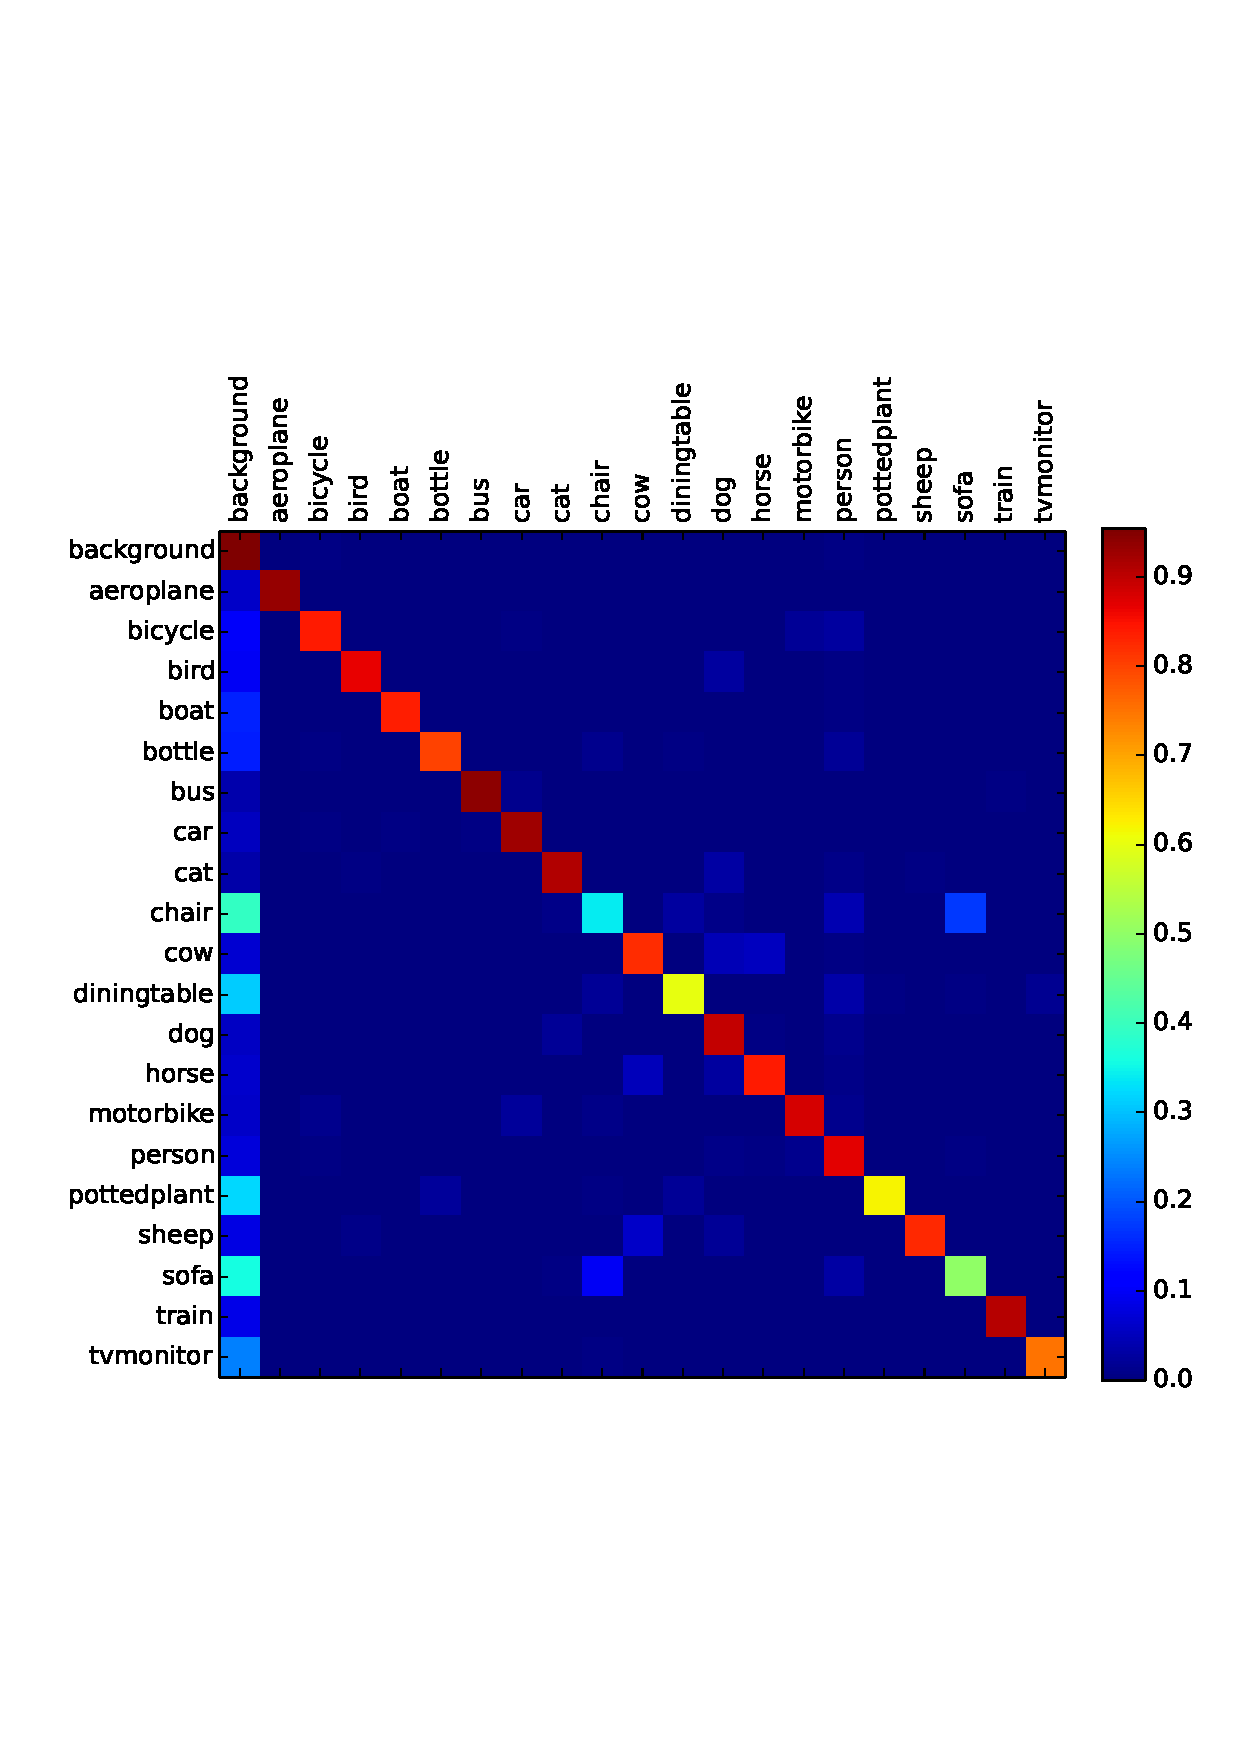
\includegraphics[width=0.5\textwidth]{image/chap04/confusion.pdf}
	\caption{镶嵌在文中的图像}
	\label{fig:image-embedding-text}
\end{wrapfigure}
论文主体是毕业论文的主要部分,必须言之成理,论据可靠,严格遵循本学科国际通行的学术规范。在写作上要注意结构合理、层次分明、重点突出,章节标题、公式图表符号必须规范统一。论文主体的内容根据不同学科有不同的特点,一般应包括以下几个方面: (1)毕业论文(设计)总体方案或选题的论证; (2)毕业论文(设计)各部分的设计实现,包括实验数据的获取、数据可行性及有效性的处理与分析、各部分的设计计算等; (3)对研究内容及成果的客观阐述,包括理论依据、创新见解、创造性成果及其改进与实际应用价值等; (4)论文主体的所有数据必须真实可靠,凡引用他人观点、方案、资料、数据等,无论曾否发表,无论是纸质或电子版,均应详加注释。自然科学论文应推理正确、结论清晰;人文和社会学科的论文应把握论点正确、论证充分、论据可靠,恰当运用系统分析和比较研究的方法进行模型或方案设计,注重实证研究和案例分析,根据分析结果提出建议和改进措施等。
论文主体是毕业论文的主要部分,必须言之成理,论据可靠,严格遵循本学科国际通行的学术规范。在写作上要注意结构合理、层次分明、重点突出,章节标题、公式图表符号必须规范统一。论文主体的内容根据不同学科有不同的特点,一般应包括以下几个方面: (1)毕业论文(设计)总体方案或选题的论证; (2)毕业论文(设计)各部分的设计实现,包括实验数据的获取、数据可行性及有效性的处理与分析、各部分的设计计算等; (3)对研究内容及成果的客观阐述,包括理论依据、创新见解、创造性成果及其改进与实际应用价值等; (4)论文主体的所有数据必须真实可靠,凡引用他人观点、方案、资料、数据等,无论曾否发表,无论是纸质或电子版,均应详加注释。自然科学论文应推理正确、结论清晰;人文和社会学科的论文应把握论点正确、论证充分、论据可靠,恰当运用系统分析和比较研究的方法进行模型或方案设计,注重实证研究和案例分析,根据分析结果提出建议和改进措施等。



\subsection{单张图像的插入}

\begin{figure}[h]
	\centering
	\includegraphics[width=0.5\textwidth]{image/chap04/illustration/hole.pdf}
	\caption{单张图像}
 	\label{fig:hole}
\end{figure}


\subsection{多张图像的并排插入}


\begin{figure}[h!]%文中的Grid-LSTM模型做的语义图像分割的例子
	\centering
	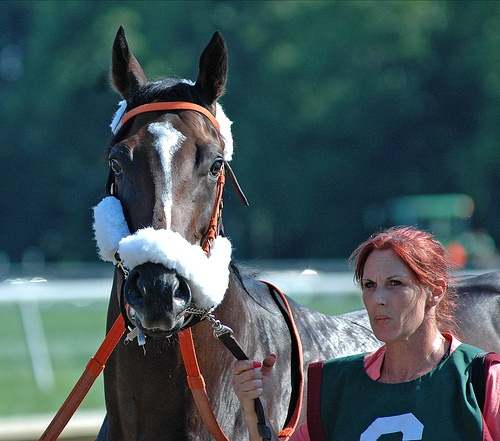
\includegraphics[width=.2\textwidth,height=.15\textwidth]{image/chap04/example/2007_000799.jpg}
	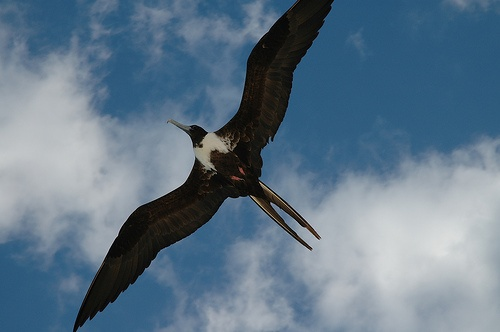
\includegraphics[width=.2\textwidth,height=.15\textwidth]{image/chap04/example/2007_002094.jpg}
	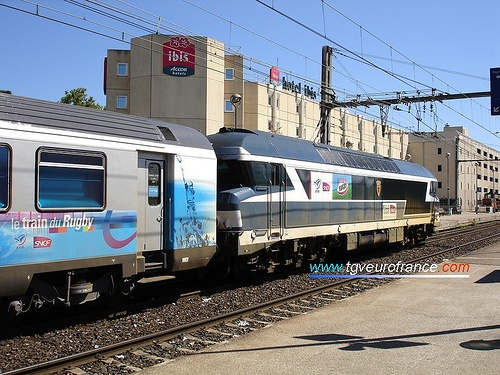
\includegraphics[width=.2\textwidth,height=.15\textwidth]{image/chap04/example/2007_004483.jpg}
	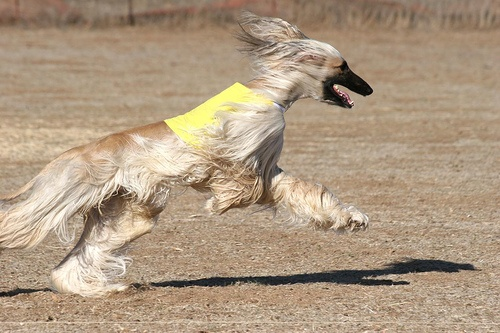
\includegraphics[width=.2\textwidth,height=.15\textwidth]{image/chap04/example/2007_003194.jpg}
	\\
	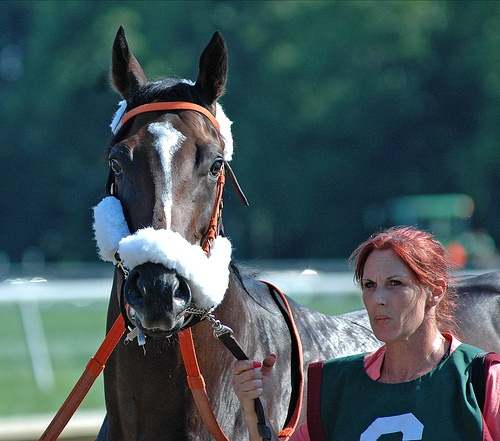
\includegraphics[width=.2\textwidth,height=.15\textwidth]{image/chap04/example/2007_000799.pdf}
	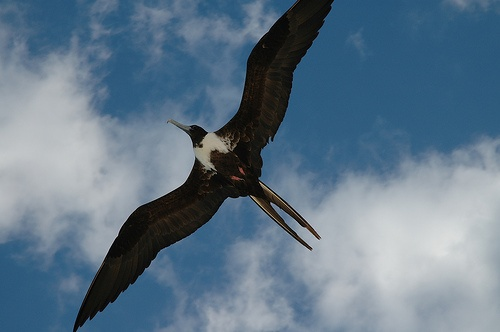
\includegraphics[width=.2\textwidth,height=.15\textwidth]{image/chap04/example/2007_002094.pdf}
	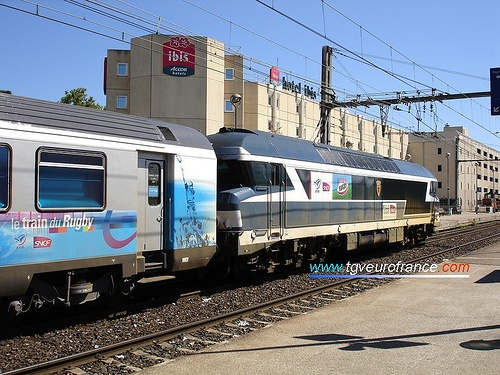
\includegraphics[width=.2\textwidth,height=.15\textwidth]{image/chap04/example/2007_004483.pdf}
	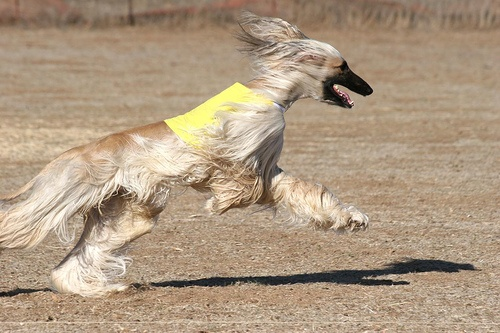
\includegraphics[width=.2\textwidth,height=.15\textwidth]{image/chap04/example/2007_003194.pdf}
	\caption{并排的多张图像}
	\label{fig:multi-image-example1}
\end{figure}


\begin{figure}[h]
	\centering
		\makebox[0.11\textwidth]{\scriptsize 图像}
		\enspace
		\makebox[0.11\textwidth]{\scriptsize 真值}
		\enspace
		\makebox[0.11\textwidth]{\scriptsize CNN+5LSTM\textbf{1}}
		\enspace\thinspace
		\makebox[0.11\textwidth]{\scriptsize CNN+5LSTM\textbf{2}}
		\enspace\thinspace
		\makebox[0.11\textwidth]{\scriptsize CNN+5LSTM\textbf{3}}
		\enspace\thinspace
		\makebox[0.11\textwidth]{\scriptsize CNN+5LSTM\textbf{4}}
		\enspace\thinspace
		\makebox[0.11\textwidth]{\scriptsize CNN+5LSTM\textbf{5}}\\
		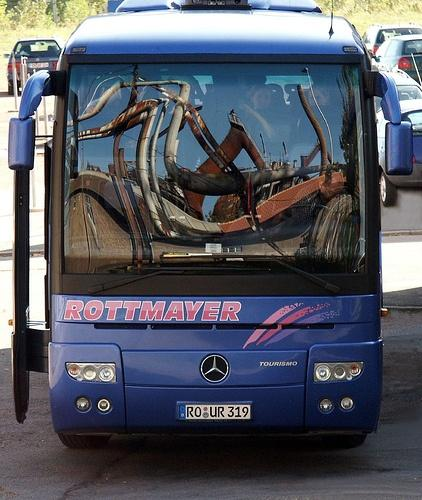
\includegraphics[width=0.11\textwidth]{image/chap04/improvement/2007_000663.jpg}
		\enspace\thinspace %\hfill
		
\includegraphics[width=0.11\textwidth]{image/chap04/improvement/2007_000663.png}
		\enspace\thinspace
		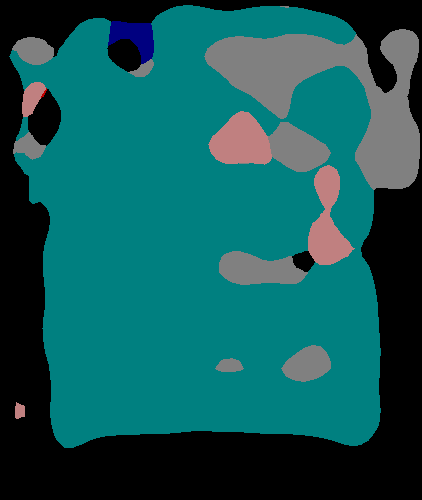
\includegraphics[width=0.11\textwidth]{image/chap04/improvement/2007_000663_1.png}
		\enspace\thinspace
		
\includegraphics[width=0.11\textwidth]{image/chap04/improvement/2007_000663_2.png}
		\enspace\thinspace
		
\includegraphics[width=0.11\textwidth]{image/chap04/improvement/2007_000663_3.png}
		\enspace\thinspace
		
\includegraphics[width=0.11\textwidth]{image/chap04/improvement/2007_000663_4.png}
		\enspace\thinspace
		
\includegraphics[width=0.11\textwidth]{image/chap04/improvement/2007_000663_5.png}
		\enspace\thinspace
		\caption{并排的多张图像加各自的注解}
		\label{fig:improvement}
\end{figure}
	

\subsection{两列图像的插入}

\begin{figure}[h!] % image examples & compare
	\begin{subfigure}{0.55\textwidth}
		\makebox[0.18\textwidth]{\scriptsize Grid-5LSTM}
		\makebox[0.18\textwidth]{\scriptsize FCN-8s\cite{long2015fully}}
		\makebox[0.18\textwidth]{\scriptsize SDS\cite{hariharan2014simultaneous}}
		\makebox[0.18\textwidth]{\scriptsize 真值}
		\makebox[0.18\textwidth]{\scriptsize 图像} \\
		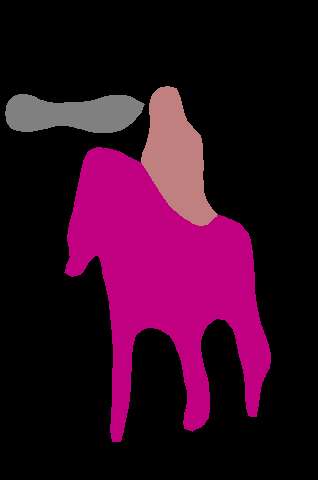
\includegraphics[width=0.18\textwidth]{image/chap04/result/compare/my_horse.pdf}
		
\includegraphics[width=0.18\textwidth]{image/chap04/result/compare/fcn_horse.png}
		
\includegraphics[width=0.18\textwidth]{image/chap04/result/compare/sds_horse.png}
		
\includegraphics[width=0.18\textwidth]{image/chap04/result/compare/gt_horse.pdf}
		\includegraphics[width=0.18\textwidth]{image/chap04/result/compare/im_horse.pdf}
		\\
		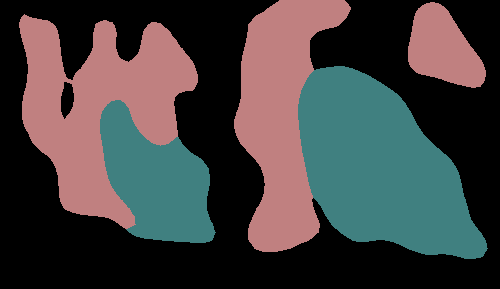
\includegraphics[width=0.18\textwidth]{image/chap04/result/compare/my_motor.png}
		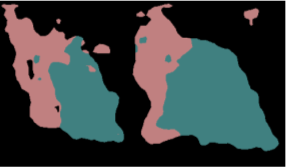
\includegraphics[width=0.18\textwidth]{image/chap04/result/compare/fcn_motor.png}
		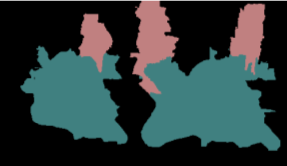
\includegraphics[width=0.18\textwidth]{image/chap04/result/compare/sds_motor.png}
		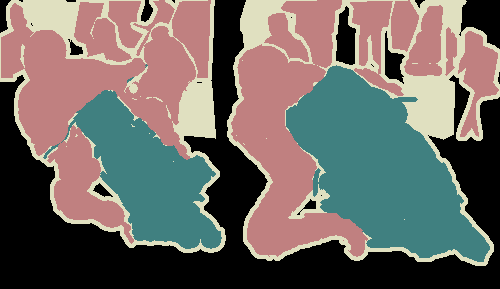
\includegraphics[width=0.18\textwidth]{image/chap04/result/compare/2007_005173.png}
		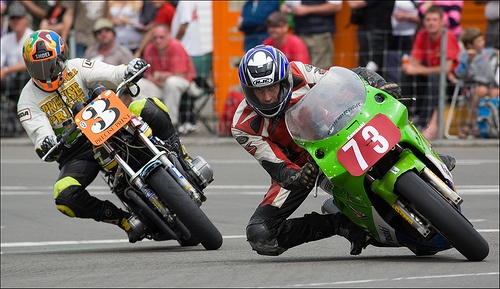
\includegraphics[width=0.18\textwidth]{image/chap04/result/compare/2007_005173.jpg}
		\\
		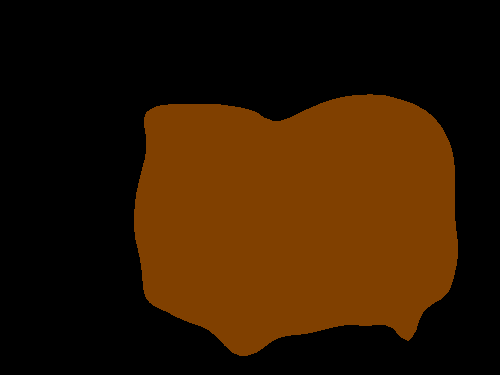
\includegraphics[width=0.18\textwidth]{image/chap04/result/compare/my_sheep.pdf}
		
\includegraphics[width=0.18\textwidth]{image/chap04/result/compare/fcn_sheep.png}
		
\includegraphics[width=0.18\textwidth]{image/chap04/result/compare/sds_sheep.png}
		\includegraphics[width=0.18\textwidth]{image/chap04/result/compare/gt_sheep.pdf}
		\includegraphics[width=0.18\textwidth]{image/chap04/result/compare/im_sheep.pdf}
		\\
		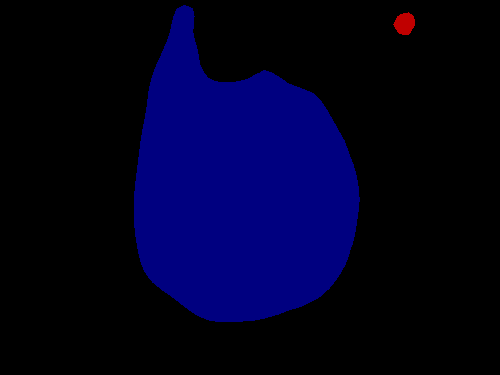
\includegraphics[width=0.18\textwidth]{image/chap04/result/compare/my_boat.png}
		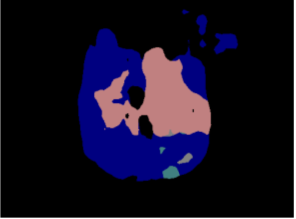
\includegraphics[width=0.18\textwidth]{image/chap04/result/compare/fcn_boat.png}
		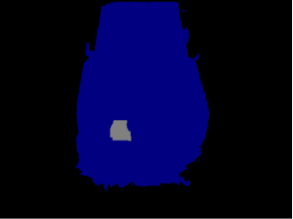
\includegraphics[width=0.18\textwidth]{image/chap04/result/compare/sds_boat.png}
		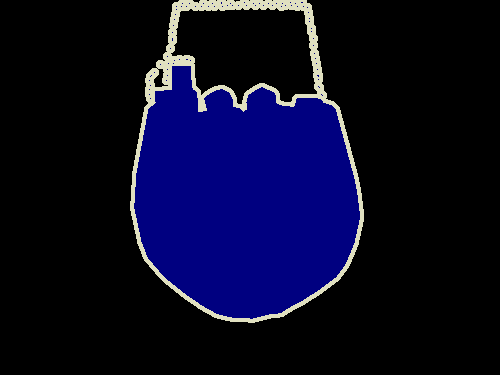
\includegraphics[width=0.18\textwidth]{image/chap04/result/compare/2007_004241.png}
		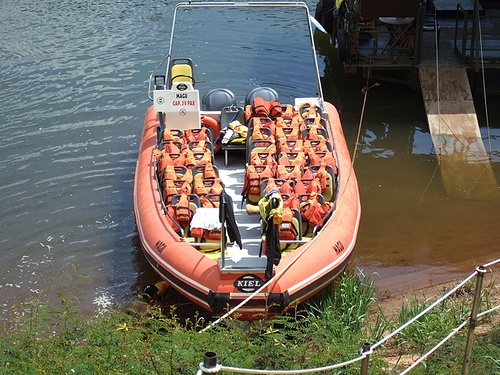
\includegraphics[width=0.18\textwidth]{image/chap04/result/compare/2007_004241.jpg}
		\caption{左边的图像}
		\label{fig:compare1}
	\end{subfigure}
	\begin{subfigure}{0.4\textwidth}
		\centering
%		\makebox[0.3\textwidth]{} \\
%		\makebox[0.3\textwidth]{} \\
		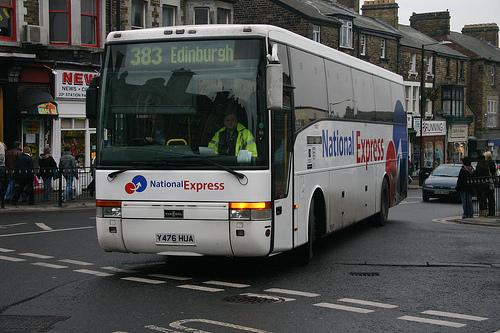
\includegraphics[width=0.25\textwidth]{image/chap04/result/compare/2010_005284.jpg}
		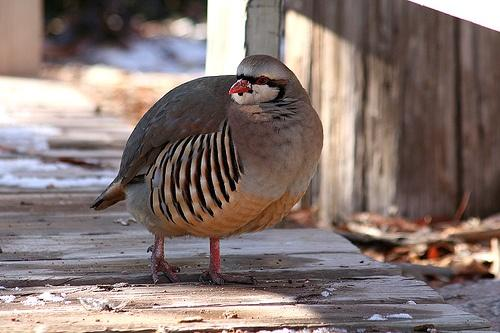
\includegraphics[width=0.25\textwidth]{image/chap04/result/compare/2007_003349.jpg}
		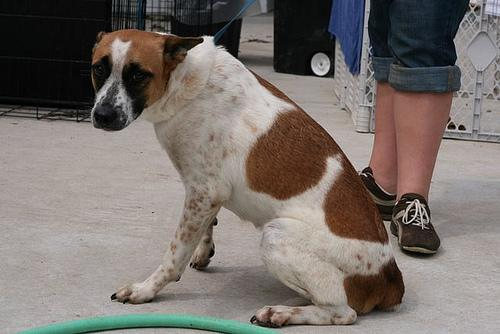
\includegraphics[width=0.25\textwidth]{image/chap04/result/compare/2009_004507.jpg} 
		\\
		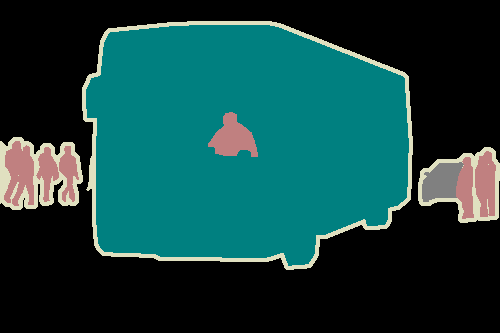
\includegraphics[width=0.25\textwidth]{image/chap04/result/compare/2010_005284.png}
		
\includegraphics[width=0.25\textwidth]{image/chap04/result/compare/2007_003349.png}
		
\includegraphics[width=0.25\textwidth]{image/chap04/result/compare/2009_004507.png} \\
		
\includegraphics[width=0.25\textwidth]{image/chap04/result/compare/zoom_bus.png}
		
\includegraphics[width=0.25\textwidth]{image/chap04/result/compare/zoom_bird.png}
		\includegraphics[width=0.25\textwidth]{image/chap04/result/compare/zoom_dog.png} \\
		\includegraphics[width=0.25\textwidth]{image/chap04/result/compare/deeplab_bus.png}
		\includegraphics[width=0.25\textwidth]{image/chap04/result/compare/deeplab_bird.png}
		\includegraphics[width=0.25\textwidth]{image/chap04/result/compare/deeplab_dog.png} \\
		\includegraphics[width=0.25\textwidth]{image/chap04/result/compare/my_bus.png}
		\includegraphics[width=0.25\textwidth]{image/chap04/result/compare/my_bird.png}
		\includegraphics[width=0.25\textwidth]{image/chap04/result/compare/my_dog.png} 
		\caption{右边的图像}
		\label{fig:compare2}
	\end{subfigure}
	\caption{复杂的两列对象的插入}
	\label{fig:complex}
\end{figure}


\clearpage

\section{表格的插入}

\begin{table}[h] %voc table result
	\centering
		\caption{典型的实验对比表格}
		\begin{tabular}{*{4}{c}}
			\toprule
	 		Method & Pixel Acc. & Mean Acc. & Mean Iu.\\
			\midrule
			Liu等人\cite{liu2011sift}  & 76.7 & - & -\\
		Tighe等人\cite{tighe2013finding}  & 78.6 & 39.2 & -\\
			FCN-16s\cite{long2015fully} & 85.2 & \textbf{51.7} & 39.5\\
			Deeplab-LargeFOV\cite{chen14semantic} & 85.6 & 51.2 & 39.7\\
			\midrule
			Grid-LSTM5 & \textbf{86.2} & 51.0 & \textbf{41.2}\\
			\bottomrule
		\end{tabular}
		\label{tab:siftflow}
\end{table}

\begin{table}[h] %voc table result
	\centering
		\caption{复杂一些的表格}
		\resizebox{\textwidth}{!}{
		\begin{tabular}{c|*{20}{c}|c}
			\toprule
			Method & aero & bike & bird & boat & bottle & bus & car & cat & chair & cow & table & dog & horse & mbike & person & plant & shep & sofa & train & tv & mIoU.\\
			\midrule
			CNN				   & 72.6 & 29.6 & 70.2 & 53.1 & 65.1 & 81.0 & 74.3 & 79.8 & 25.0 & 64.8 & 47.8 & 69.5 & 66.2 & 65.2 & 74.2 & 42.1 & 69.6 & 38.8 & 74.4 & 58.6 & 62.5\\
			CNN+\textbf{1}LSTM & 71.5 & 30.6 & 70.5 & 53.8 & 64.9 & 82.4 & 77.1 & 79.5 & 25.1 & 65.8 & 47.8 & 71.5 & 64.6 & 67.0 & 74.0 & 43.9 & 69.6 & 38.6 & 74.9 & 59.4 & 63.0\\
			CNN+\textbf{2}LSTM & 76.1 & 32.6 & 72.1 & 57.0 & 65.3 & 83.6 & 75.4 & 81.7 & 24.7 & 69.3 & 47.5 & 72.3 & 68.9 & 69.5 & 74.7 & 41.5 & 69.8 & 38.3 & 77.8 & 62.1 & 64.3 \\
			CNN+\textbf{3}LSTM & 77.7 & 32.3 & 72.6 & 60.0 & 68.3 & 85.5 & 78.5 & 82.3 & 25.3 & 71.1 & 49.7 & 71.5 & 69.7 & 70.8 & 75.9 & 47.9 & 71.2 & 38.9 & 80.2 & 61.7 & 65.8 \\
			CNN+\textbf{4}LSTM & 79.1 & \textbf{33.7} & \textbf{73.6} & \textbf{62.0} & \textbf{70.4} & 85.5 & \textbf{80.9} & 83.7 & \textbf{24.1} & 70.7 & 45.7 & 73.7 & 69.6 & 72.1 & 75.6 & 47.2 & \textbf{76.0} & 37.3 & 80.5 & 62.2 & 66.4 \\
			CNN+\textbf{5}LSTM & \textbf{79.9} & 33.6 & \textbf{73.6} & 61.7 & 68.0 & \textbf{88.5} & \textbf{80.9} & \textbf{84.0} & 23.6 & \textbf{71.3} & \textbf{49.7} & \textbf{73.1} & \textbf{71.3} & \textbf{72.9} & \textbf{76.4} & \textbf{48.9} & 75.1 & \textbf{38.1} & \textbf{84.5} & \textbf{63.8} & \textbf{67.2} \\
			\midrule
			CNN+\textbf{5}LSTM$^\dag$ & 84.8 & 36.4 & 82.0 & 69.4 & 73.0 & 87.2 & 81.8 & 86.1 & 34.5 & 82.4 & 53.1 & 81.5 & 77.4 & 79.0 & 81.3 & 54.8 & 81.1 & 47.0 & 84.3 & 67.3 & 72.3 \\
			\bottomrule
		\end{tabular}}
		\label{tab:vocval}
	\end{table}
	

\section{公式}
\label{sec:formula}
没有编号的公式
\begin{align*}
\begin{split}
	\label{eq:feedforward}
	\mybold{z}^{(l)} & = \mybold{W}^{(l)}\mybold{a}^{(l-1)} + \mybold{b}^{(l)} \\
	\mybold{a}^{(l)} & = f(\mybold{z}^{(l)})
\end{split}
\end{align*}
公式中含有中文
\begin{align}
	\begin{split}
	\mbox{像素准确率} &= \sum_{i=1}^{n_{cl}}n_{ii} / \sum_{i=1}^{n_{cl}}t_i \\
		\mbox{平均像素准确率} &= \frac{1}{n_{cl}} \sum_{i=1}^{n_{cl}}(n_{ii}/ t_i) \\
	\mbox{Mean IU} &= \frac{1}{n_{cl}} \sum_{i=1}^{n_{cl}}\frac{n_{ii}}{t_i + \sum_j^{n_{cl}} n_{ji} - n_{ii}}
	\end{split}
\end{align}
公式中含有矩阵
\begin{equation}
	\textbf{H} = \begin{bmatrix}
		I*\mybold{x}_i \\ \textbf{h}
	\end{bmatrix}
\end{equation}
每行后面都有编号的公式
\begin{align}
	\frac{\partial}{\partial W_{ij}^{(l)}} J(\mybold{W},\mybold{b};\mybold{x},y) &= \frac{\partial J(\mybold{W},\mybold{b};\mybold{x},y)}{\partial z_i^{(l+1)}}\cdot \frac{\partial z_i^{(l+1)}}{\partial W_{ij}^{(l)}} = \delta_i^{(l+1)}a_j^{(l)} \\
	\frac{\partial}{\partial b_i^{(l)}} J(\mybold{W},\mybold{b};\mybold{x},y) &= \frac{\partial J(\mybold{W},\mybold{b};\mybold{x},y)}{\partial z_i^{(l+1)}}\cdot \frac{\partial z_i^{(l+1)}}{\partial b_i^{(l)}} = \delta_i^{(l+1)}
\end{align}

\section{算法流程图}
\label{sec:algorithm}
\begin{algorithm}[h]
\KwIn{$m$个训练样本}
\lFor{$l=1$ \emph{\KwTo} $n_l$}{
初始化:$\Delta \mybold{W}^{(l)}=0$,$\Delta \mybold{b}^{(l)}=0$}
\ForEach{训练样本}{
	\lFor{$l=1$ \emph{\KwTo} $n_l-1$}{
	前向传播:$\mybold{z}^{(l+1)}=\mybold{W}^la^l+\mybold{b}^l$,$\mybold{a}^{(l+1)}=f(\mybold{z}^{(l+1)})$}
	输出误差计算:$\delta^{(n_l)} = \frac{\partial}{\partial \mybold{z}^{(n_l)}} J(\mybold{W},\mybold{b};\mybold{x},y)$\;
	\lFor{$l=n_l-1$ \emph{\KwTo} $1$}{
	后向传播:$\delta^{(l)} = \bigl((\mybold{W}^{(l)})^T \delta^{(l+1)}\bigr)f'(\mybold{z}^{(l)})$}
	\ForAll{层l}{
		计算梯度:$\nabla_{\mybold{W}^{(l)}}J(\mybold{W},\mybold{b};\mybold{x},y)=\delta^{(l+1)}(\mybold{a}^{(l)})^T$ \\
		\hspace{60pt}$\nabla_{\mybold{b}^{(l)}}J(\mybold{W},\mybold{b};\mybold{x},y)=\delta^{(l+1)}$\;
		累加梯度:$\Delta \mybold{W}^{(l)} \leftarrow \Delta \mybold{W}^{(l)} + \nabla_{\mybold{W}^{(l)}}J(\mybold{W},\mybold{b};\mybold{x},y)$; \\
		\hspace{60pt}$\Delta \mybold{b}^{(l)} \leftarrow \Delta \mybold{b}^{(l)} + \nabla_{\mybold{b}^{(l)}}J(\mybold{W},\mybold{b};\mybold{x},y)$\;
	}
}
\ForAll{层$l$}{
	更新权重:$\mybold{W}^{(l)} \leftarrow \mybold{W}^{(l)} - \alpha \biggl[\frac 1m \Delta \mybold{W}^{(l)}\biggr]$ \\
	\hspace{60pt} $\mybold{b}^{(l)} \leftarrow \mybold{b}^{(l)} - \alpha \biggl[\frac 1m \Delta \mybold{b}^{(l)}\biggr]$
}
\caption{梯度下降算法}
\label{algo:sgd}
\end{algorithm}

\section{例子、定理与证明}

\begin{eg}
  这是一个例子, 用以验证特殊环境的字体成功更改为楷体.
\end{eg}

\begin{theorem}[定理例子]
	\label{the:example-theorem}
	这是一个定理。
\end{theorem}

\begin{corollary}[推论例子]
	\label{the:example-corollary}
	这是一个推论。
\end{corollary}

\begin{lemma}[引理例子]
	\label{the:example-lemma}
	这是一个引理。
\end{lemma}

这里我们先给出\autoref{the:example-theorem-sysu-thesis}

\begin{theorem}[中山大学毕业论文模板定理]
\label{the:example-theorem-sysu-thesis}
中山大学 \LaTeX 毕业论文模板\cite{sysu-thesis}可以用于写各种证明。
\end{theorem}

下面我们对\autoref{the:example-theorem-sysu-thesis}进行证明:


\begin{proof}

下面我们开始证明:

由本定理的证明可见,我可以引用\autoref{the:example-theorem}和引理\ref{the:example-corollary}以及推论\ref{the:example-lemma}来证明我这个 \LaTeX 可以用来写各种证明。 \\

\autoref{the:example-theorem-sysu-thesis}得证。
\end{proof}



\section{其他的一些用法}
\label{sec:font}
\subsection{子章节编号}
\label{sec:font:subsection}
\subsubsection{更小的章节}
\label{sec:font:subsection:subsub}
更小的章节编号也是支持的。

可以如此引用章节:

\begin{itemize}
	\item \autoref{cha:usage-example}
	\item  \autoref{sec:font}
	\item  \autoref{sec:font:subsection}
	\item  \autoref{sec:font:subsection:subsub}
\end{itemize}


\subsection{列表的使用}
\label{sec:font:list}

这是一个无序列表
\begin{itemize}
	\item 引用文献\cite{long2015fully}
	\item 字体{\color{red}{变红}},\textbf{粗体},\textit{斜体},\underline{下划线}。
\end{itemize}

这是一个有序列表
\begin{enumerate}
	\item 索引前面的\autoref{sec:formula}、图像\ref{fig:complex}、表格\ref{tab:siftflow}
	\item 加脚注\footnote{测{\zihao{-5}试一下}脚注和URL \url{http://cs231n.github.io/transfer-learning/}}
\end{enumerate}



\section{总结与展望}
\subsection*{总结与展望}
\frame{
   \footnotesize
	\begin{block}{工作总结}
	\begin{itemize}
		\item[\dag] 本文的模型结合了卷积网络的特征学习能力与长短记忆网络对整体局部建模的能力,相比于全卷积网络,大幅度地提高了了模型性能
		\item[\dag] 大量的对比实验与结果分析证明了模型的有效性 
	\end{itemize}
	\end{block}
	\vspace{-1em}
	\begin{block}{展望}
	\begin{itemize}
		\item[\dag] 模型性能:提高网络的深度来学习更高层次的特征,提高模型效果(He et al. ResNet, CVPR 2016)
		\item[\dag] 模型大小:通过裁剪网络冗余部分(Han et al. Deep Compression, ICLR 2016 Best Paper)或使用二值网络减少模型参数(Courbariaux et al. Binaryconnect, NIPS 2015)
		\item[\dag] 训练数据:使用无监督或弱监督的方式训练网络(Papandreou et al. Weakly-and semi-supervised learning, ICCV 2015)
	\end{itemize}
	\end{block}
}



\section{致谢}
\subsection*{致谢}
\frame{
	\frametitle{致谢}
	\begin{block}{我的感谢}
		\begin{itemize}
			\item 首先要感谢数院给我来这里修读双学位的机会
			\item 感谢我的指导老师的悉心指导
			\item 感谢同学的帮助、家人的支持
			\item 感谢答辩委员会的倾听和指导
		\end{itemize}
	\end{block}
	\vspace{-1em}
	\note{
		我的展示到此结束,我要感谢我的指导老师,家人还有答辩委员会老师的倾听与指导。谢谢大家
	}
}
\frame{
	\frametitle{Q \& A}
	\begin{block}{Questions?}
		~\\ ~\\
		\center{\Large{Thank you!}}
		\\ ~\\ ~\\ ~\\ ~\\
	\end{block}
	\note{
		现在是问答时间。请问老师们对我的展示有什么疑问?
	}
}



\end{document}
